\documentclass[11pt,letterpaper,twoside,english]{article}

\usepackage[margin=1.4in]{geometry} % controls the size of the margins

% Special symbols, etc.
\usepackage{amssymb,amsbsy,latexsym,ytableau}
\usepackage{amsmath}
\usepackage{graphics, subfigure, float} 
\usepackage{cancel}
%\usepackage{todonotes}
% Encoding settings
\usepackage[latin1]{inputenc}
\usepackage[american]{babel}
\usepackage[T1]{fontenc} 
\usepackage{tikz}

\usepackage{titling} % allows posttitle command

% AMS Math packages

\usepackage{amscd,amsthm}

\usepackage{verbatim, comment} % can comment out text 
\usepackage{mdwlist} 

% Graphics
%\usepackage[dvips]{graphicx,epsfig,color}
%\usepackage{subfigure}
%\usepackage{pst-all}
%\usepackage{pstricks-add}
\usepackage{hyperref}  % can only be used with pdflatex - gives hyperlinks
\usepackage{bm} % bold math font
\usepackage{bbm}
\usepackage{todonotes}

\newtheoremstyle{theorem}{1em}{1em}{\slshape}{0pt}{\bfseries}{.}{ }{}
\theoremstyle{theorem}
\newtheorem{theorem}{Theorem}
\newtheorem*{theorem*}{Theorem}
\newtheorem{corollary}[theorem]{Corollary}
\newtheorem{proposition}[theorem]{Proposition}
\newtheorem{lemma}[theorem]{Lemma}
\newtheorem{claim}[theorem]{Claim}
\newtheorem{conjecture}[theorem]{Conjecture}
\newtheorem{definition}[theorem]{Definition}
\newtheorem*{claim*}{Claim}

\theoremstyle{remark}
\newtheorem{remark}{Remark}
\newtheorem*{remark*}{Remark}
\newtheorem{algorithm}{Algorithm}
\newtheorem*{question*}{Question}
\newtheorem{question}{Question}
\newtheorem{example}{Example}

\providecommand{\setN}{\mathbb{N}}
\providecommand{\setZ}{\mathbb{Z}}
\providecommand{\setQ}{\mathbb{Q}}
\providecommand{\setR}{\mathbb{R}}
\providecommand{\E}{\mathrm{E}}
\providecommand{\Pr}{\mathrm{Pr}}
\providecommand{\Var}{\mathrm{Var}}

\tikzset
{
    treenode/.style = {circle, draw=black, align=center, minimum size=1cm},
}

\makeatother

\title{Avoidance in permutations} 

\author{Yajit Jain, Deepak Narayanan, Leon Zhang}

\begin{document}

\maketitle

\section{Introduction}

In this paper we will investigate pattern avoidance in permutations of finite sets of the first $n$ positive integers for arbitrary $n$.

Before beginning our discussion, we present the following definitions.

\begin{definition}
Two finite sequences $a_1,\cdots a_k$ and $b_1,\cdots b_k$ have the same relative order if the $i^\text{th}$ largest entry of each unordered set $\{a_1,\cdots,a_k\}$ and $\{b_1,\cdots, b_k\}$ appears in the same position in $a_1\cdots a_k$ and $b_1\cdots b_k$ for each $1\le i\le k$. 
\end{definition}

\begin{definition}
A finite sequence of numbers $a_1a_2\cdots a_n$ avoids a sequence $b_1\cdots b_k$ with $n\ge k$ if no subsequence $a_{i_1}a_{i_2}\cdots a_{i_k}$ of $a_1a_2\cdots a_n$ has its terms in the same relative order as $b_1\cdots b_k$. 
\end{definition}

\begin{example}
The sequence 15432 avoids 123 while the sequence 13425 does not. The latter example fails because 134 appears in 15342 with the same relative order as 123. 
\end{example}


\begin{remark}
Let $S_n$ be the set of permutations of $\{1,\cdots, n\}$. There are two conventions commonly used to write elements of $S_n$. The first is $\emph{one-line}$ notation where permutations in $S_n$ are written explicitly, e.g. 43215 is a permutation of $\{1,2,3,4,5\}$ in $S_5$. 

The second is \emph{cycle notation}, where a cycle $(a_1\cdots a_n)\in S_n$ with $1\le a_i\le n$ acts on a sequence by sending $a_1\mapsto a_2$, $a_2\mapsto a_3$, $\cdots$, $a_n\mapsto a_1$. For example, the cycle $(14)(23)$ sends $12345$ to $43215$. Unless otherwise stated, we will refer to permutations in one-line notation. 
\end{remark}

\begin{definition} 
A permutation $\sigma\in S_n$ avoids a permutation $\pi\in S_k$ if the sequence of numbers for the one-line notation for $\sigma$ avoids the sequence of numbers for the one-line notation for $\pi$.
\end{definition}

\begin{definition}
For a permutation $\pi\in S_k$, $s_n(\pi)$ represents the number of permutations in $S_n$ that avoid $\pi$. 
\end{definition}

In this paper we concern ourselves with the sequence of numbers $s_n(\pi)$ for various $\pi$. In section \ref{S3} we will consider sequence $s_n(\pi)$ for $\pi\in S_3$, and prove that the sequence $s_n(\pi)$ for all such $\pi$ is in fact the sequence of Catalan numbers. In section \ref{S4} we will consider sequence $s_n(\pi)$ for $\pi\in S_4$. In section \ref{Tn} we consider a variation on the avoidance problem that considers the problem of avoiding sequences in a subset $T_n$ of $S_n$. 

\subsection{Generating Trees}

Before continuing we introduce generating trees, a tool we can use to study pattern avoidance. The generating tree for the sequence $s_n(\pi)$ is the infinite tree whose vertices are elements of $S_n$ that avoid $\pi$. To construct the tree, we define the children of an arbitrary node. Let $\omega\in S_k$ be a node of the generating tree of $s_n(\pi)$. Then the children of $\omega$ are elements of $S_{k+1}$ that avoid $\pi$ and that can be obtained by inserting the integer $k+1$ between integers in $\omega$. Figure \ref{fig:M1} is an example of the generating tree of $s_n(312)$. 

\begin{figure}[h!]
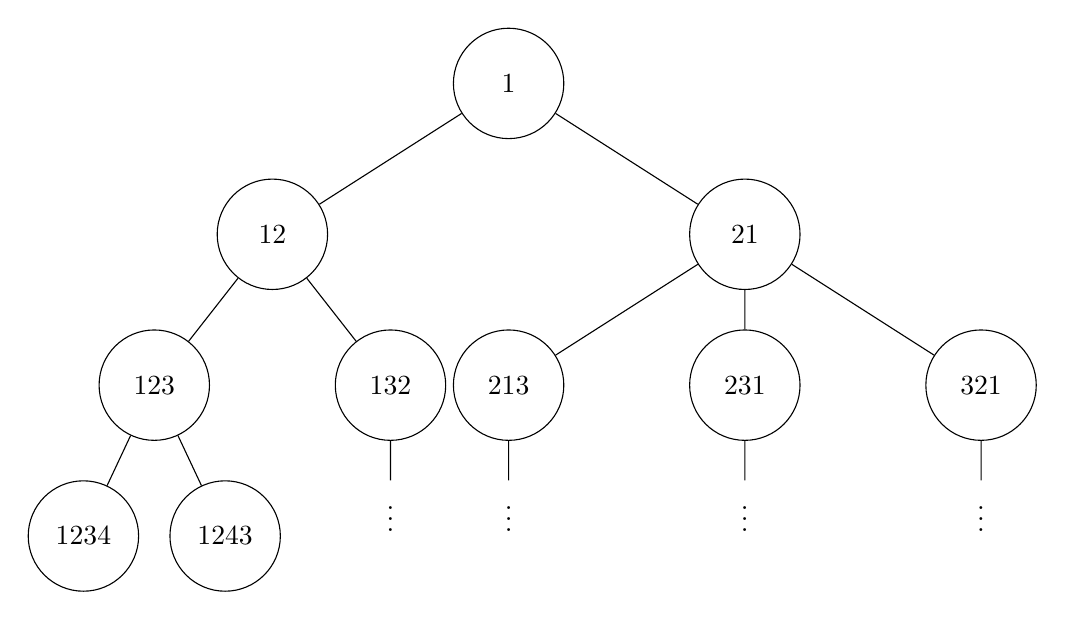
\begin{tikzpicture}[level distance=0.5cm, growth parent anchor={south}, nodes={anchor=north}]
\tikzstyle{hollow node}=[circle,draw,inner sep=0.1mm, text width=1.36cm,align=center]
\tikzstyle{level 1}=[sibling distance=6cm] 
\tikzstyle{level 2}=[sibling distance=3cm] 
\tikzstyle{level 3}=[sibling distance=1.8cm]
\tikzstyle{level 4}=[sibling distance=0.9cm]
\node [hollow node]{1}
	child {
		node[hollow node] {12}
		child{
			node[hollow node]{123}
			child{node[hollow node]{1234}}
			child{node[hollow node]{1243}}
		}
		child{
			node[hollow node]{132}
			child{node{\vdots}}
		}
	}
    	child {
		node[hollow node] {21}
    		child {
			node[hollow node] {213}
			child{node{\vdots}}
		}
      		child {
			node[hollow node] {231}
			child{node{\vdots}}
		}
		child {
			node[hollow node] {321}
			child{node{\vdots}}
		}
    	};

\end{tikzpicture}
\caption{Generating tree of the sequence $s_n(312)$} \label{fig:M1}
\end{figure}

\subsection{Flipping}
Another notion that we will use in this paper is the concept of `flipping'. We define the \emph{flip} of a sequence $a$ as the sequence $b$ with the same elements as $a$, but with the largest element swapped with the smallest element, the second largest element swapped with the second smallest element, etc. For example, the flip of 1324 is 4321. We will discuss the flip as it becomes useful.

\section{Terms in the sequence $s_n(312)$}
\label{S3}

We claim that the sequence of numbers $s_n(312)$ is in fact the sequence of Catalan numbers. We state this result formally as the following theorem,

\begin{theorem}
The total number of permutations of $\{1,2,3,...,n\}$ that avoid the order $312$ as a subsequence is $C_n$ where $C_n$ is the $n^{th}$ Catalan number.
\end{theorem}

Before proving the theorem, we state and prove the following lemma, that will be used in our proof of the theorem.
\begin{lemma}
\label{lemma1}
All permutations of $\{1,2,\dots,k,k+1\}$ ending in $i$ that avoid the order $312$ as a sub-sequence must be of the form,
$$\pi_1 \pi_2 i$$
where $\pi_1$ is a permutation of $\{1,2,\ldots,(i-1)\}$ that avoids the order $312$ as a sub-sequence and $\pi_2$ is a permutation of $\{(i+1),\ldots,(k+1)\}$ that avoids the order $312$ as a sub-sequence.
\end{lemma}

\begin{proof}
It is clear that any subsequences of the permutation $\pi = \pi_1 \pi_2 i$ must avoid $312$ if the entire permutation $\pi$ is to avoid $312$ as well; this implies that the permutations $\pi_1$ and $\pi_2$ must avoid $312$ as well.

We proceed with a proof by contradiction.

Before proceeding, we define the sets $A$ and $B$ to be $\{1,2,\ldots,(i-1)\}$ and $\{(i+1),(i+2),\ldots,(k+1)\}$ respectively. For the sake of contradiction, let us assume that there exists some permutation $\pi$ of $\{1,2,...,k,k+1\}$ that ends with value $i$ such that some integer $x < i$ (that is, $x \in A$) is to the right of some integer $y > i$ ($y \in B$). Clearly, this permutation is not of the form described above. It is also easy to see that $\pi$ does \emph{not} avoid the order $312$ since the triple $(y, x, i)$ satisfies the condition $y > x > i$ and is in the order $312$.

From this we conclude that all $x < i$ must be to the left of all $y > i$. This information coupled with the fact that we are only considering permutations that end with $i$ complete the claim that only permutations of the form described above can avoid $312$.

\end{proof}

With this lemma proven, we move on to the proof of our theorem.

\begin{proof}
The inductive hypothesis holds for our base case of $\{1\}$, since the only permutation of $\{1\}$ trivially avoids $312$.

Now, we need to prove the inductive case. Let us first assume that for all $i$ from $1$ to $k$, the number of permutations of $\{1,2,...,i\}$ that avoid the order $312$ as a subsequence is $C_i$.

Now, we want to prove the inductive hypothesis for $\{1,2,...,k,k+1\}$ as well, that is the number of permutations of $\{1,2,...,k,k+1\}$ that avoid the order $312$ as a subsequence is $C_{k+1}$.

We count the number of permutations of $\{1,2,...,k,k+1\}$ that avoid $312$ by enumerating through all possible values of the last term of a valid permutation.
If the last term of the permutation is $i$ (where $i \in \{1,2,...,k,k+1\}$), then let us define the subsets $A$ and $B$ of the  set $\{1,2,...,k+1\} \setminus \{i\}$ as the set of integers less than $i$ and the set of integers greater than $i$ respectively. It is clear from the definition of $A$ and $B$ that $A$ and $B$ are disjoint from each other.

Now, from the above lemma, we know that all permutations of $\{1,2,...,k,k+1\}$ ending in $i$ that avoid $312$ must be of the form,

$$\pi = \pi_1 \pi_2 i$$

where $\pi_1$ is a permutation of $A$ that avoids the order $312$ as a sub-sequence and $\pi_2$ is a permutation of $B$ that avoids the order $312$ as a sub-sequence. It is clear that the above permutation contains all integers between $1$ and $k+1$, from the definitions of the subsets $A$ and $B$, which implies that $\pi_1\pi_2i$ is permutation of the set $\{1,2,...,k,k+1\}$.

Now, the total number of permutations $\pi$ is,
$$n_{\pi_1} \cdot n_{\pi_2} = C_{i-1} \cdot C_{k-i+1}$$
since the total number of valid permuations $\pi_1$ is simply going to be $C_{i-1}$ (total number of valid permutations of length $i-1$ that avoid the order $312$ as a sub-sequence is $C_{i-1}$; similarly $n_{\pi_2} = C_{k-1+1}$)

Now, summing over all possible values of $i$, we see that the total number of permutations of $\{1,2,...,k+1\}$ that avoid $312$ is equal to,
$$\sum_{i=1}^{k+1} C_{i-1} \cdot C_{k-i+1} = \sum_{i=0}^k C_i \cdot C_{k-i}$$ which is in fact $C_{k+1}$, and we are done.

\end{proof}

It is easy to see that the above proof can be modified slightly to prove that the sequences $s_n(132)$, $s_n(213)$ and $s_n(231)$ are in fact the sequence of catalan numbers as well. In fact, we claim that if $\sigma$ and $\pi$ are both permutations in $S_k$ for some arbitrary $k$, then if $\sigma = flip(\pi)$, $s_n(\pi) = s_n(\sigma)$. This is easy to see since if $a$ is a permutation that avoids $\sigma$, then $flip(a)$ is a permutation that avoids $\pi$ -- since this can be done both ways, it is bijective and we can conclude that the cardinalities of the two sets are equal, or $s_n(\sigma) = s_n(\pi)$.

\section{Terms in the sequence $s_n(321)$}

Unfortunately, there is no clear way to reformulate Lemma \ref{lemma1} for the case of avoiding the permutation 321 or 123. As a consequence, the proof in the previous section simply does not hold. Fortunately, however, we still have a closed form expression for $s_n(321)$ (recall that $s_n(321)=s_n(123)$ by our flipping principle). Surprisingly, in fact, the sequence remains the same: $s_n(321)=C_n$, the $n^{th}$ Catalan number. In order to prove this result, however, we will need the machinery of Young tableaux. What follows is a brief exposition of the key results, adapted from Stanley's \emph{Algebraic Combinatorics}.

\begin{definition}
A Young diagram of a partition $\lambda=\{\lambda_1, \lambda_2, \ldots, \lambda_n\}$ of the integer $\sum_{i=1}^n \lambda_i$ is a left-justified array of squares, with $\lambda_i$ squares in the $i$th row.
\end{definition}
\begin{example}
The Young diagram of $(4, 3, 1, 1)$ looks like:
\[
\ytableausetup{centertableaux}
\begin{ytableau}
\ & \ & \ & \ \\
\ & \ & \ \\
\ \\
\
\end{ytableau}
\]
\end{example}

\begin{definition}
A standard Young tableau (or SYT) consists of the Young diagram $D$ of some partition $\lambda$ of an integer $n$, together with the numbers $1, 2, \ldots, n$ inserted into the squares of $D$, so that each number appears exactly once, and every row and column is \emph{increasing}. We call $\lambda$ the \emph{shape} of the SYT.
\end{definition}

\begin{example}
There are five SYT of the shape $(2, 2, 1)$. They are given by
\[\ytableausetup{aligntableaux=top}
\begin{ytableau}
1 & 2 \\
3 & 4\\
5
\end{ytableau}\ \ \ \ \
\hfill
\begin{ytableau}
1 & 2 \\
3 & 5\\
4
\end{ytableau}\ \ \ \ \
\hfill
\begin{ytableau}
1 & 3 \\
2 & 4\\
5
\end{ytableau}\ \ \ \ \
\hfill
\begin{ytableau}
1 & 3 \\
2 & 5\\
4
\end{ytableau}\ \ \ \ \
\hfill
\begin{ytableau}
1 & 4 \\
2 & 5\\
3
\end{ytableau}.\]
\end{example}

\begin{definition}
Let $u$ be a square of the Young diagram of the partition $\lambda$. Then the hook $H(u)$ is the set of all squares directly to the right of $u$ or directly below $u$, including $u$ itself. The size of $H(u)$ is called the hook length of $u$, and is denoted $h(u)$.
\end{definition}

\begin{example}
In the Young diagram of the partition $(4, 2, 2)$ below, each square $u$ contains its hook length $h(u)$.
\[\ytableausetup{centertableaux}
\begin{ytableau}
6 & 5 & 2 & 1\\
3 & 2\\
2 & 1
\end{ytableau}\]
\end{example}

\begin{theorem}
Let $\lambda$ be a partition of $n$. Then $f^\lambda$, the number of SYT of shape $\lambda$, is given by
\[f^\lambda=\frac{n!}{\prod_{u\in \lambda} h(u)},\]
where the notation $u\in \lambda$ means that $u$ ranges over all squares of the Young diagram of $\lambda$.
\end{theorem}

The theorem above is called the \emph{hook-length formula}.

\begin{example}
The diagram above for the hook lengths of $\lambda=(4, 2, 2)$ tells us that the number of SYT of shape $\lambda$ is given by
\[\frac{8!}{6\cdot 5\cdot 2 \cdot 1 \cdot 3 \cdot 2 \cdot 2\cdot 1}=56.\]
\end{example}

It is an easy application of the hook-length formula to prove the following theorem:

\begin{theorem}
The number of SYT of shape $(n, n)$ is given by $C_n$, the $n^{th}$ Catalan number.
\end{theorem}

We need only one more result before we are ready to prove our central result.

\begin{theorem}
There exists an algorithm (called the \emph{RSK algorithm}) which defines a bijection between the set of permutations in $S(n)$ avoiding a decreasing subsequence of length 3 and the set of pairs of size-$n$ SYT of the same shape and at most two rows. 
\end{theorem}
Using all this machinery and all these results, we are finally able to prove the closed-form expression for $s_n(321)$.
\begin{theorem}
The total number of permutations of $\{1,2,3,\ldots, n\}$ that avoid the order 321 as a subsequence is $C_n$, where $C_n$ is the $n^{th}$ Catalan number.
\end{theorem}
\begin{proof}
By the first part of Theorem 12, there are $s_n(321)$ elements in the set $A$ of pairs of size-$n$ SYT of the same shape and at most two rows. By Theorem 11, the set $B_n$ of SYT of shape $(n, n)$ has its size given by $C_n$. We will construct a bijection between the sets $A_n$ and $B_n$: because $|A_n|=s_n(321)$ and $|B_n|=C_n$, it will therefore follow that $s_n(321)=C_n$, as desired.

Given any pair of size $n$ Young tableaux of the same shape and at most two parts, take the second tableau and invert its numbers: that is, send $i$ to $2n+1-i$ for all $i$. Now rotate the Young tableau and `fit' it into the first tableau. We demonstrate this process for a pair of Young tableaux with $n=6$: we begin with
\[\ytableausetup{aligntableaux=top}
\begin{ytableau}
1 & 2 &3&4\\
5 & 6
\end{ytableau} \ \ \ \ \ 
\hfill
\begin{ytableau}
1 & 3 & 4 & 5\\
2 & 6
\end{ytableau}.\]
Inverting the numbers of the second tableau gives us
\[\ytableausetup{aligntableaux=top}
\begin{ytableau}
1 & 2 &3&4\\
5 & 6
\end{ytableau} \ \ \ \ \ 
\hfill
\begin{ytableau}
12 & 10 & 9 & 8\\
11 & 7
\end{ytableau}.\]
Finally, rotating the second Young tableau and fitting it into the first gives us
\[\ytableausetup{aligntableaux=top}
\begin{ytableau}
1 & 2 &3&4&7&11\\
5 & 6&8&9&10&12
\end{ytableau},\]
a valid Young tableau of shape $(6, 6)$. 

Beginning with a pair of size $n$ Young tableaux of shape $\lambda$ and at most two parts, it is easy to see that this process always yields a valid Young tableau of shape $(n, n)$. Indeed, we can also define the inverse: given any Young tableau for the partition $(n, n)$, we can find the shape formed by all numbers greater than $n$: split it off from the original tableau, rotate it, and invert the numbers to get a pair of size $n$ Young tableau of the same shape and at most two parts. These processes can be easily checked to be inverses: hence the two sets are of the same size, and the proof follows.
\end{proof}

\section{Conjectures on $s_n(\pi)$ for $\pi\in S_4$}
\label{S4}

In this section we will present our findings and conjectures about sequences $s_n(\pi)$ for $\pi\in S_4$. We computed values up to $s_{10}$. It appears that there are three sequences that appear, and we have sorted the permutations according to which sequence they produce and paired them with their flips.  

We define the following sequences based on the first 8 terms:
$$
A:=1,2,6,23,103,512,2740,15485,91245\ldots
$$
$$
B:=1,2,6,23,103,513,2761,15767,94359\ldots
$$
$$
C:=1,2,6,23,103,513,2762,15793,94776\ldots
$$

The table below lists the elements of $S_4$ generate sequences $A,B,C$ for the first 8 terms.

\begin{center}
\begin{tabular}{|c|c|c|}
B &A&C\\
\hline
1234, 4321&4132, 1423&4231,1324\\
1243, 4312&4213, 1342&\\
1432, 4123&2431,3124&\\
2134, 3421&2413, 3142&\\
2143, 3412&2314, 3241&\\
2341, 3214&&\\
\end{tabular}
\end{center}

There is no guarantee that these sequences will not diverge and produce more than three distinct sequences, however for now we hypothesize that $A$, $B$, and $C$ are the only sequences that arise for $s_n(\pi)$ with $\pi\in S_4$. Assuming this hypothesis, if we write each length four permutation in cycle notation, a pattern begins to emerge. 

\begin{center}
\begin{tabular}{|c|c|c|}
B &A&C\\
\hline
(1),(14)(23)&(243),(142)&(23),(14)\\
(34),(1423)&(234),(143)&\\
(24),(1432)&(124),(132)&\\
(12),(1324)&(123),(134)&\\
(12)(34),(13)(24)&(1243),(1342)&\\
(1234),(13)&&\\
\end{tabular}
\end{center}

So we conjecture that sequence $A$ is characterized by elements of $S_4$ that are three cycles or four cycles when written in cycle notation. Sequence $B$ seems to be characterized by either a pair of disjoint two cycles paired with a flip that is a 2-cycle, or a single 4-cycle paired with a flip that is a 2-cycle. Sequence $C$ appears to be characterized by a 2-cycle paired with a 2-cycle as a flip. 


\section{Avoidance of permutations of $T_n$}
\label{Tn}
We now impose further restrictions on the set of permutations $S_n$. This new set of permutations, $T_n$ is defined follows.

\begin{definition}
For even $n$, $T_n$ is defined as the set of all permutations $\sigma \in S_n$ for which $1,3,5,\ldots,2n-1$ appear in increasing order, and $2i$ always appears to the right of $2i-1$.
\end{definition}

Since $T_n$ is only defined for even $n$, henceforth we shall refer to $T_n$ as $T_{2m}$ where $m$ is any integer greater than or equal to $0$.

Given the above definition of $T_{2m}$, we prove the following result about the cardinality of $T_{2m}$.

\begin{theorem}
$|T_{2m}| = 1 \cdot 3 \cdot 5 \cdot \ldots \cdot (2m-1)$
\end{theorem}

\begin{proof}
Observe that since $1,3,5,\ldots,2m-1$ must appear in increasing order in $T_{2m}$, our problem is now reduced to determining the relative order of $2,4,6,\ldots,2m$ with respect to each other, as well as with respect to $1,3,5,\ldots,2m-1$.

Let us first try to insert $2m$ into the sequence $1,3,5,\ldots,2m-1$. Clearly, the way $T_{2m}$ is defined, $2m$ can be inserted into only $1$ slot, the one following $2m-1$. (Here we define a slot as a gap between two existing elements of the sequence, or the gap that follows the last element of the sequence or the gap that precedes the first element of the sequence)

Now, let us try to insert $(2m-2)$ into the sequence. $(2m-2)$ can be inserted into $3$ slots in the sequence -- the one between $2m-3$ and $2m-1$, the one between $2m-1$ and $2m$ or the one following $2m$.

Now, if we try to insert $(2m-4)$ into this incompletely formed sequence, we will see that there are $5$ possible locations into which this number can be inserted. Continuing this for all even numbers upto $2$, we observe that the total number of ways such a sequence can  be created is equal to $1 \cdot 3 \cdot 5 \cdot \ldots \cdot (2m-1)$, as desired.
\end{proof}

Studying avoidance of permutations in $T_n$ seems an interesting exercise. In the following section, we consider the sequence of numbers $t_n(\pi)$, defined as the number of permutations in $T_n$ that avoid the permutation $\pi$. In particular, we consider permutations $\pi \in S_3$.

Before stating our conjectures, we present the computed sequences. Note that since the sequence $T_n$ is defined only for even $n$, we only present the even terms of the sequence $t_n$.

$$t_n(123) = 1, 0, 0, 0, 0, \ldots$$
$$t_n(132) = 1, 1, 1, 1, 1, \ldots$$
$$t_n(213) = 1, 2, 4, 8, 16, \ldots$$
$$t_n(231) = 1, 2, 4, 8, 16, \ldots$$
$$t_n(312) = 1, 3, 12, 55, 273, \ldots$$
$$t_n(321) = 1, 3, 12, 55, 273, \ldots$$

It is easy to see why $t_n(123)$ and $t_n(132)$ behave the way they do -- since all odd numbers in $T_n$ are increasing, it is impossible to have a permutation in $T_n$ that avoids $123$ and the permutation consisting of all increasing integers is the only permutation of $T_n$ that avoids $132$.

More interesting is the equivalences between $213$ and $231$, and $312$ and $321$. We will prove the equivalence between $312$ and $321$ below, but before doing so, we first state and prove the following lemmas which will be useful in our proof.

\begin{lemma}
\label{tn_avoidance}
If $a$ and $b$ are two elements that appear in a permutation in $T_n$ such that $a$ is to the left of $b$, then if $a > b$, $b$ must be even.
\end{lemma}

\begin{proof}
For the sake of contradiction, let us assume that $b$ is odd. Then there exist two possibilities that need to be considered -- one, that $a$ is odd, and two, that $a$ is even.

\begin{itemize}
\item \textbf{Case 1:} $a$ is odd.

Note that all permutations in $T_n$ must have odd elements monotonically increasing. So if $a$ appears to the left of $b$, and both $a$ and $b$ are odd, then $a$ must be less than $b$ -- a contradiction. Hence, we conclude that $a$ can't be odd.

\item \textbf{Case 2:} $a$ is even.

For all permutations $\sigma$ in $T_n$, every even element $j$ must be to the right of all odd elements less than $j$. From this, we conclude that since $a$ is even, it must be to the right of all odd numbers less than it. But $b$ is an odd number less than $a$ -- we conclude that $a$ can't be even either.
\end{itemize}

Since $a$ can't be odd or even if $b$ is odd, we conclude that $b$ must be even, as desired.
\end{proof}

\begin{lemma}
\label{swapping_lemma}
If $x, y, z$ is a three-element subsequence of a permutation $\pi$ in $T_n$ such that $x > y > z$ or $x > z > y$, then swapping $y$ and $z$ in the permutation $\pi$ yields a permutation $\pi'$ that also belongs to $T_n$.
\end{lemma}

\begin{proof}
From Lemma \ref{tn_avoidance} we see that both $y$ and $z$ must be even. Then there exist two cases that need to be covered.
\begin{itemize}
\item \textbf{Case 1:} $x$ is odd.

If $x$ is odd, then it is clear that the permutation $\pi'$ obtained from swapping $y$ and $z$ is still valid, since both $y$ and $z$ are to the right of the odd numbers $y-1$ and $z-1$ (since $y-1$ and $z-1$ are themselves to the left of $x$ since they are strictly less than $x$)

\item \textbf{Case 2:} $x$ is even.

If $x$ is even, then $x-1$ which is an odd number greater than both $y-1$ and $z-1$, must be to the left of $x$. Since $y-1$ and $z-1$ are already to the left of $x-1$, we conclude that swapping $y$ and $z$ still ensures that $y$ and $z$ are both to the right of $y-1$ and $z-1$.
\end{itemize}
Hence, we see that regardless of whether $x$ is even or odd, swapping $y$ and $z$ in a permutation $\pi \in T_n$ if $x > y > z$ or $x > z > y$ yields a permutation $\pi'$ that also belongs to $T_n$.
\end{proof}

Given these lemmas, we now present a proof for $t_n(312) = t_n(321)$.

\begin{theorem}
$t_n(312) = t_n(321)$
\end{theorem}

\begin{proof}
First observe from Lemma \ref{tn_avoidance} that if $x, y, z$ is a subsequence of three elements of a permutation in $T_n$ in the relative order $312$ or $321$, then both $y$ and $z$ must be even.

We now construct a bijective mapping between all permutations in $T_n$ that avoid $312$ and all permutations in $T_n$ that avoid $321$.

Consider a permutation $\pi$ in $T_n$ that avoids $312$. For each permutation $\pi \in T_n$ that avoids $312$, we want to show that there exists a sequence of transformation moves that transforms $\pi$ to a unique permutation $\pi'$ that avoids $321$.

\textbf{May want to skip the transformation stuff, and directly talk about the bijection being established.}

If the original permutation $\pi$ avoids $321$ already, then clearly $\pi' = \pi$ avoids $321$.

Now if $\pi$ does not avoid $321$, there must exist some sub-sequence $x, y, z$ in $\pi$ in the relative ordering $321$. From Lemma \ref{swapping_lemma}, we see that swapping $y$ and $z$ in the permutation $\pi$ yields another valid permutation $\pi_1$ in $T_n$ -- note that the permutation produced after this swap has $x, y, z$ in the relative ordering $312$ instead of $321$. Note that $\pi_1$ may still have sub-sequences in the relative ordering $321$, so we may have to perform the above swapping operation again to get some permutation $\pi_2 \in T_n$ such that a sub-sequence $x_1, y_1, z_1$ in $\pi_1$ that has a relative ordering $321$ is in the relative ordering $312$ in $\pi_2$. Continuing this process produces the following chain of permutations,
$$\pi \rightarrow \pi_1 \rightarrow \pi_2 \rightarrow \ldots \rightarrow \pi_k$$
Where the last permutation in the chain $\pi_k$ does not have a single three-element sub-sequence in the relative ordering $321$, that is $\pi' = \pi_k$ is a permutation in $T_n$ that avoids $321$.

This process is completely invertible, since we can take a permutation $\pi'$ in $T_n$ that avoids $321$, and traverse through the above chain in reverse order to obtain a permutation that avoids $312$.

What remains to be proven is that the order of swapping operations in the chain of transformations does not matter -- that is, any valid transformation chain starting with some permutation $\pi \in T_n$ that avoids $312$, will always produce the same permutation $\pi' \in T_n$ that avoids $321$. Note that since we're only swapping even elements, the odd elements are in exactly the same position in both $\pi$ and $\pi'$. In addition, for every element $i \in \pi$, all even numbers in $\pi$ to the right of $i$ and less than $i$ must be in decreasing order; in $\pi'$, for every element $i \in \pi'$, all even numbers in $\pi'$ to the right of $i$ and less than $i$ must be in increasing order.

Since there exists a bijective mapping between permutations in $T_n$ that avoid $312$ and permutations in $T_n$ that avoid $321$, we can conclude that $t_n(312) = t_n(321)$.

\end{proof}

Unfortunately, it turns out that proving the equivalence between $231$ and $213$ is not as straightforward as above, partially due to the fact that the element corresponding to $2$ and $3$ in the above sub-sequences can be either even or odd, which means we now also have to account for the positions of odd elements too. Proving this equivalence remains future work.

\end{document}